\paragraph{QuizziPedia::Front-End::Directives::SignUpBarDirective}

\label{QuizziPedia::Front-End::Directives::SignUpBarDirective}
\begin{figure} [ht]
	\centering
	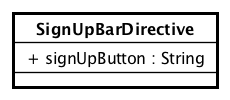
\includegraphics[scale=0.80]{UML/Classi/Front-End/QuizziPedia_Front-end_Directives_SignUpBarDirective.png}
	\caption{QuizziPedia::Front-End::Directives:SignUpBarDirective}
\end{figure} \FloatBarrier
\begin{itemize}
	\item \textbf{Descrizione}: directive contenente il componente che permette di effettuare il redirect alla pagina di registrazione;
	\item \textbf{Utilizzo}: permette di effettuare il redirect alla pagina di registrazione;
	\item \textbf{Relazioni con altre classi}:
	\begin{itemize}
		\item \textbf{IN \texttt{MenuBarModelView}}: classe di tipo \textit{modelview\ped{G}} la cui istanziazione è contenuta all'interno della variabile di ambiente \$scope di \textit{Angular\ped{G}}. All'interno di essa sono presenti le variabili e i metodi necessari per il \textit{Two-Way Data-Binding\ped{G}} tra la \textit{view\ped{G}} \texttt{Index} e il \textit{controller\ped{G}} \texttt{MenuBarController};
		\item \textbf{OUT \texttt{MenuBarDirective}}: rappresenta il menù, presente in ogni pagina dell'applicazione, generato in base agli oggetti passati nello \$scope isolato. Fornisce un pulsante per ogni oggetto ricevuto come parametro, ogni pulsante viene rappresentato con un’icona e con un testo. Al click di un pulsante viene invocata la funzione ad esso associata.  
	\end{itemize}
	\item \textbf{Attributi}:
	\begin{itemize}
		\item \texttt{+ signUpButton: String} \\ Attributo che viene utilizzato per visualizzare la giusta traduzione della \textit{label\ped{G}} per il bottone di link alla registrazione, in italiano o inglese.
	\end{itemize}
\end{itemize}